%%%%%%%%%%%%%%%%%%%%%%%%%%%%%%%%%%%%%%%%%
% Short Sectioned Assignment LaTeX Template Version 1.0 (5/5/12)
% This template has been downloaded from: http://www.LaTeXTemplates.com
% Original author:  Frits Wenneker (http://www.howtotex.com)
% License: CC BY-NC-SA 3.0 (http://creativecommons.org/licenses/by-nc-sa/3.0/)
%%%%%%%%%%%%%%%%%%%%%%%%%%%%%%%%%%%%%%%%%

%----------------------------------------------------------------------------------------
%	PACKAGES AND OTHER DOCUMENT CONFIGURATIONS
%----------------------------------------------------------------------------------------

\documentclass[paper=a4, fontsize=11pt]{scrartcl} % A4 paper and 11pt font size

% ---- Entrada y salida de texto -----

\usepackage[T1]{fontenc} % Use 8-bit encoding that has 256 glyphs
\usepackage[utf8]{inputenc}
\usepackage{fourier} % Use the Adobe Utopia font for the document - comment this line to return to the LaTeX default

% ---- Idioma --------

\usepackage[spanish, es-tabla]{babel} % Selecciona el español para palabras introducidas automáticamente, p.ej. "septiembre" en la fecha y especifica que se use la palabra Tabla en vez de Cuadro

% ---- Otros paquetes ----
\usepackage{array}
\usepackage{multirow}
\usepackage[dvipsnames]{xcolor}
\usepackage{url} % ,href} %para incluir URLs e hipervínculos dentro del texto (aunque hay que instalar href)
\usepackage{amsmath,amsfonts,amsthm, tikz,dsfont} % Math packages
\usepackage[hidelinks]{hyperref}
%\usepackage{graphics,graphicx, floatrow} %para incluir imágenes y notas en las imágenes
\usepackage{graphics,graphicx, float, listings} %para incluir imágenes y colocarlas

% Para hacer tablas comlejas
%\usepackage{multirow}
%\usepackage{threeparttable}

%\usepackage{sectsty} % Allows customizing section commands
%\allsectionsfont{\centering \normalfont\scshape} % Make all sections centered, the default font and small caps

\usepackage{fancyhdr} % Custom headers and footers
\pagestyle{fancyplain} % Makes all pages in the document conform to the custom headers and footers
\fancyhead{} % No page header - if you want one, create it in the same way as the footers below
\fancyfoot[L]{} % Empty left footer
\fancyfoot[C]{} % Empty center footer
\fancyfoot[R]{\thepage} % Page numbering for right footer
\renewcommand{\headrulewidth}{0pt} % Remove header underlines
\renewcommand{\footrulewidth}{0pt} % Remove footer underlines
\setlength{\headheight}{13.6pt} % Customize the height of the header

\numberwithin{equation}{section} % Number equations within sections (i.e. 1.1, 1.2, 2.1, 2.2 instead of 1, 2, 3, 4)
\numberwithin{figure}{section} % Number figures within sections (i.e. 1.1, 1.2, 2.1, 2.2 instead of 1, 2, 3, 4)
\numberwithin{table}{section} % Number tables within sections (i.e. 1.1, 1.2, 2.1, 2.2 instead of 1, 2, 3, 4)

\setlength\parindent{0pt} % Removes all indentation from paragraphs - comment this line for an assignment with lots of text

\newcommand{\horrule}[1]{\rule{\linewidth}{#1}} % Create horizontal rule command with 1 argument of height


%----------------------------------------------------------------------------------------
%	TÍTULO Y DATOS DEL ALUMNO
%----------------------------------------------------------------------------------------

\title{	
\normalfont \normalsize 
\textsc{\textbf{Sistemas Operativos (2017-2018)} \\ Grado en Ingeniería Informática \\ Universidad de Granada} \\ [25pt] % Your university, school and/or department name(s)
\horrule{0.5pt} \\[0.4cm] % Thin top horizontal rule
\huge Guión Practicas \\ % The assignment title
\horrule{2pt} \\[0.5cm] % Thick bottom horizontal rule
\begin{figure}[H] %con el [H] le obligamos a situar aquí la figura
	\centering
	
\includegraphics[scale=0.5]{image/ugr.png}  %el parámetro scale permite agrandar o achicar la imagen. En el nombre de archivo puede especificar directorios
\end{figure}
}

\author{Antonio Rodríguez Alaminos} % Nombre y apellidos

\date{\normalsize\today} % Incluye la fecha actual

%----------------------------------------------------------------------------------------
% DOCUMENTO
%----------------------------------------------------------------------------------------

\begin{document}

%----------------------------------------------------------------------------------------
% PORTADA
%----------------------------------------------------------------------------------------

\maketitle % Muestra el Título

\newpage %inserta un salto de página

\tableofcontents % para generar el índice de contenidos

%----------------------------------------------------------------------------------------
% INDICE
%----------------------------------------------------------------------------------------

\listoffigures

\listoftables

\newpage

\part[Módulo 2]{Módulo 2: Uso de los Servicios del SO mediante la API}

\section[Sesion 1]{Sesion 1: Llamadas al sistema para el SA(Parte 1)}

{\Large \textbf{Ejercicio 1.}} ¿Qué hace el siguiente programa? Probad tras la ejecución del programa las siguientes órdenes del shell: \$ > cat archivo y \$ > od -c archivo. \href{file: file/tarea1.c}{\textcolor{Blue}{Descarga file}}


\lstset{language=C, breaklines=true, basicstyle=\footnotesize}
\begin{lstlisting}[frame=single]

#include<unistd.h>
#include<stdio.h>
#include<stdlib.h>
#include<sys/types.h>  	
#include<sys/stat.h>
#include<fcntl.h>
#include<errno.h>

char buf1[]="abcdefghij";
char buf2[]="ABCDEFGHIJ";

int main(int argc, char *argv[]) {
	int fd;
	
	//Parte A
	if((fd=open("archivo",O_CREAT|O_TRUNC|O_WRONLY,S_IRUSR|S_IWUSR))<0) {
		printf("\nError %d en open",errno);
		perror("\nError en open");
		exit(EXIT_FAILURE);
	}
	//Parte B
	if(write(fd,buf1,10) != 10) {
		perror("\nError en primer write");
		exit(EXIT_FAILURE);
	}
	//Parte C
	if(lseek(fd,40,SEEK_SET) < 0) {
		perror("\nError en lseek");
		exit(EXIT_FAILURE);
	}
	//Parte D
	if(write(fd,buf2,10) != 10) {
		perror("\nError en segundo write");
		exit(EXIT_FAILURE);
	}

	return EXIT_SUCCESS;
}

\end{lstlisting}

Este programa lo que hace es almacenar las dos cadenas de caracteres una tras otra en un archivo denominado ``archivo''. Esto se realiza en los siguientes etapas o partes del programa: \newline

\textbf{Parte A:} En esta parte el programa abre (si no existe lo genera) el fichero archivo. En caso de tener algún problema, nos informara de él mediante un mensaje, este es generado por la función perror: ``Error en open''.\newline

\textbf{Parte B:} En este apartado se escribirá la cadena \textit{buf1} (``abcdefghij'') al inicio del archivo abierto o generado ``archivo''. Si se produce algún error, el programa como antes, gracias a la función perror genera un mensaje de error: ``Error en el primer write''.\newline

\textbf{Parte C:} Ahora continua realiza un desplazamiento del contador del buffer de lectura del archivo que tenemos abierto. Si sucede algún error perror no devuelve: ``Error en lseek''. \newline

\textbf{Parte D:} Se almacena en el fichero el \textit{buf2}, en caso contrario perror nos avisa con: ``Error en segundo write''. \newline

Ahora que ya tenemos generado el fichero ``archivo pasamos a la segunda parte del ejercicio. Como podemos observar parece que las cadenas se almacenaron una seguida de la otra. \newline

\begin{figure}[h]
	\centering
	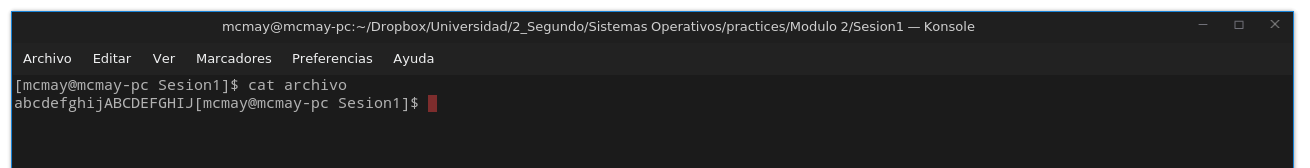
\includegraphics[width=1\linewidth]{image/ejer-01-A}
	\caption[Ejercicio 1. A]{Resultado obtenido tras ejecutar \$cat archivo}
	\label{fig:ejer01a}
\end{figure}

Pero como podemos ver con el siguiente comando esto no es de verdad lo que ha sucedido, ya que en este caso podemos ver como esta separadas una de otras por una cadena de 40 caracteres vacíos. \newline

\begin{figure}[h]
	\centering
	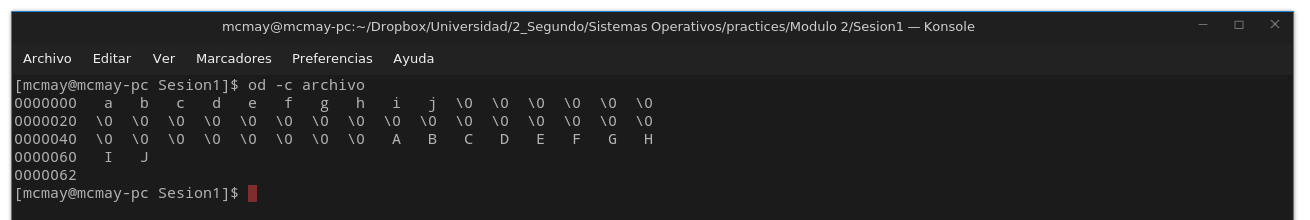
\includegraphics[width=1\linewidth]{image/ejer-01-B}
	\caption[Ejercicio 1. B]{Resultado obtenido tras ejecutar \$od -c archivo}
	\label{fig:ejer01b}
\end{figure}

\newpage

{\Large \textbf{Ejercicio 2.}} Implementa un programa que realice la siguiente funcionalidad. El programa
acepta como argumento el nombre de un archivo (pathname), lo abre y lo lee en bloques de
tamaño 80 Bytes, y crea un nuevo archivo de salida, salida.txt, en el que debe aparecer la
siguiente información:

\lstset{language=, breaklines=true, basicstyle=\footnotesize}
\begin{lstlisting}[frame=single]
Bloque 1
//Aqui van los primeros 80 Bytes del archivo pasado como argumento.
Bloque 2
//Aqui van los segundos 80 Bytes del archivo pasado como argumento.
...
Bloque n
//Aqui van los siguientes 80 Bytes del archivo pasado como argumento.
\end{lstlisting}

Si no se pasa un argumento al programa se debe utilizar la entrada estándar como archivo de entrada. \newline

{\Large \textbf{Modificación adicional.}} ¿Cómo tendrías que modificar el programa para que una vez
finalizada la escritura en el archivo de salida y antes de cerrarlo, pudiésemos indicar en su
primera línea el número de etiquetas ''Bloque i'' escritas de forma que tuviese la siguiente
apariencia?: \href{file: file/ejercicio_2.c}{\textcolor{Blue}{Descarga file}}


\lstset{language=, breaklines=true, basicstyle=\footnotesize}
\begin{lstlisting}[frame=single]
	El numero de bloques es <nº_bloques>
\end{lstlisting}

Aquí tenemos el código que se desarrolla para el programa solicitado. 

\lstset{language=, breaklines=true, basicstyle=\footnotesize}
\begin{lstlisting}[frame=single]

#include<unistd.h>
#include<stdio.h>
#include<stdlib.h>
#include<sys/types.h>   
#include<sys/stat.h>
#include<fcntl.h>
#include<errno.h>

int main(int argc, char const *argv[]) { 
	//declaramos los ficheros que utilizaremos
	int fread, fwrite, numbytestmp = 0, contador = 1;
	char buffer[80];
	
	
	//comprobamos los argumentos pasados al programa  
	if(argc < 2) {
		fread = STDIN_FILENO;
	}else{
		//apertura o generacion del fichero de salida
		if((fread=open(argv[1],O_RDONLY)) < 0) {
			perror("\nError en open read");
			exit(EXIT_FAILURE);
		}
	}
	
	
	
	
	//apertura o generacion del fichero de salida
	if((fwrite=open("salida.txt",O_CREAT|O_TRUNC|O_WRONLY,S_IRUSR|S_IWUSR)) < 0) {
		perror("\nError en open write");
		exit(EXIT_FAILURE);
	}
	
	//reservamos un trozo para el codigo que se requiere introducir al final
	if(lseek(fwrite,80,SEEK_SET) < 0) {
		perror("\nError en el desplazamiento(lseek)");
		exit(EXIT_FAILURE);
	}
	
	//lectura mientras de pueda del fichero se almacena en ftmp
	while ((numbytestmp = read(fread, &buffer, 80)) > 0){
		//introducimos el numero de bloque
		char titulo[16];
		if((sprintf(titulo, "\nBloque %i \n", contador)) < 0){
			perror("\nError en la inserción del titulo");
			exit(EXIT_FAILURE);
		}
		if (write(fwrite, &titulo, sizeof(titulo)) < 0) {
			perror("\nError en el write de la inserción del tituto ");
			exit(EXIT_FAILURE);
		}
		
		//pasamos a introducir los 80 bytes correspondientes por bloque
		if ((write(fwrite, &buffer, numbytestmp)) < 0) {
			perror("\nError en la inserción del buffer");
			exit(EXIT_FAILURE);
		}
		
		contador++;
	}
	
	//introducimos el titulo inicial
	char buffer2[40];
	if((sprintf(buffer2, "El número de bloques total es de: %i.\n", contador-1)) < 0){
		perror("\nError en la inserción del titulo inicial.");
		exit(EXIT_FAILURE);
	}
	if(lseek(fwrite,0,SEEK_SET) < 0){
		perror("\nError en el desplazamiento de la inserción del titulo final.");
		exit(EXIT_FAILURE);
	}
	if((write(fwrite, &buffer2, sizeof(buffer2))) < 0) {
		perror("\nError en la inserción del titulo final.");
		exit(EXIT_FAILURE);
	}
	
	
	
	
	//cerramos los fichero abiertos
	close(fread);
	close(fwrite);
	
	return EXIT_SUCCESS;
}
\end{lstlisting}

Capturas de pantalla que muestran lo sucedido al ejecutar el programa introduciendo como argumento el código del ejercicio anterior. \newline

\begin{figure}[H]
	\centering
	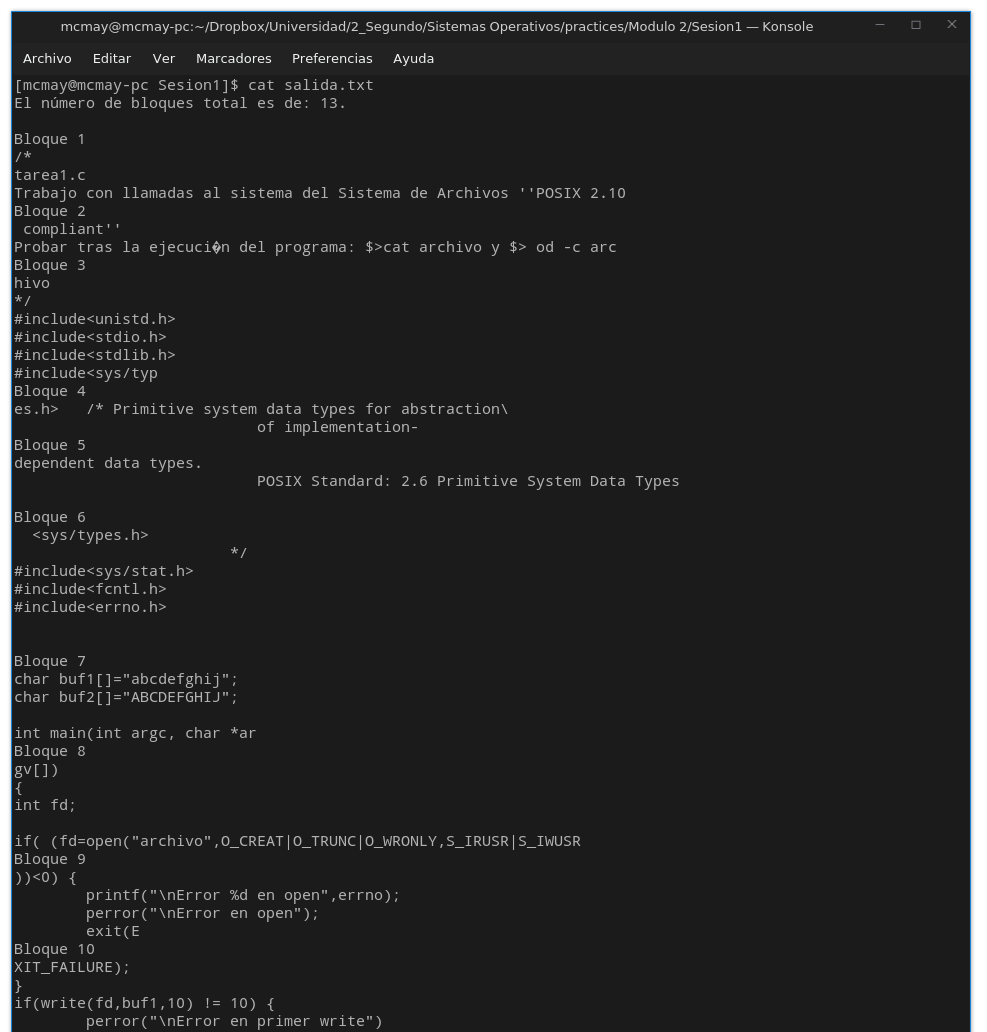
\includegraphics[width=0.9\linewidth]{image/ejer-02-A}
	\caption[Ejercicio 2. A]{Primera parte de la muestra por pantalla del ejercicio.}
	\label{fig:ejer-02-a}
\end{figure}

\begin{figure}[H]
	\centering
	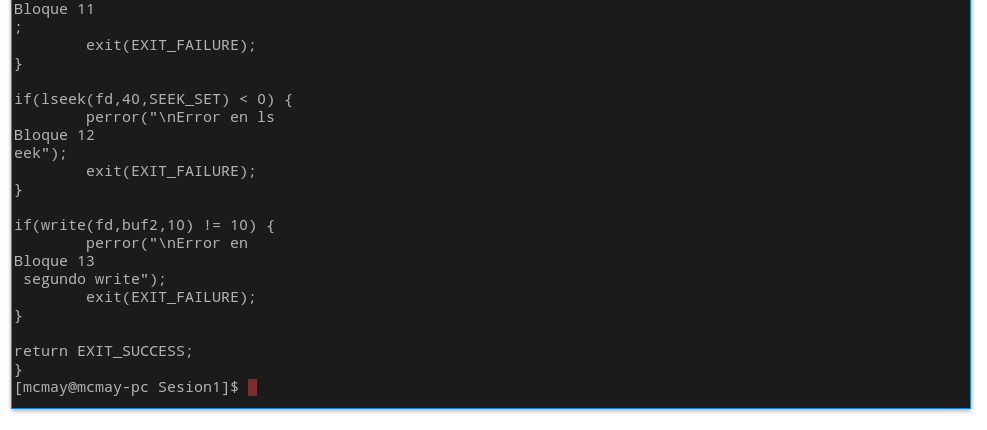
\includegraphics[width=1\linewidth]{image/ejer-02-B}
	\caption[Ejercicio 2. B]{Primera parte de la muestra por pantalla del ejercicio.}
	\label{fig:ejer-02-b}
\end{figure}

{\Large \textbf{Ejercicio 3.}} ¿Qué hace el siguiente programa? \href{file: file/tarea2.c}{\textcolor{Blue}{Descarga file}}

\lstset{language=, breaklines=true, basicstyle=\footnotesize}
\begin{lstlisting}[frame=single]

#include<unistd.h>  
#include<stdio.h>
#include<stdlib.h>
#include<sys/types.h>  
#include<sys/stat.h>
#include<stdio.h>
#include<errno.h>
#include<string.h>

int main(int argc, char *argv[])
{
	int i;
	struct stat atributos;
	char tipoArchivo[30];
	
	//Parte A
	if(argc<2) {
		printf("\nSintaxis de ejecucion: tarea2 [<nombre_archivo>]+\n\n");
		exit(EXIT_FAILURE);
	}
	
	for(i=1;i<argc;i++) {
		//Parte B
		printf("%s: ", argv[i]);
		if(lstat(argv[i],&atributos) < 0) {
			printf("\nError al intentar acceder a los atributos de %s",argv[i]);
			perror("\nError en lstat");
		}
		
			
		//Parte C		
		else {
			if(S_ISREG(atributos.st_mode)) strcpy(tipoArchivo,"Regular");
			else if(S_ISDIR(atributos.st_mode)) strcpy(tipoArchivo,"Directorio");
			else if(S_ISCHR(atributos.st_mode)) strcpy(tipoArchivo,"Especial de caracteres");
			else if(S_ISBLK(atributos.st_mode)) strcpy(tipoArchivo,"Especial de bloques");
			else if(S_ISFIFO(atributos.st_mode)) strcpy(tipoArchivo,"Tuberia con nombre (FIFO)");
			else if(S_ISLNK(atributos.st_mode)) strcpy(tipoArchivo,"Enlace relativo (soft)");
			else if(S_ISSOCK(atributos.st_mode)) strcpy(tipoArchivo,"Socket");
			else strcpy(tipoArchivo,"Tipo de archivo desconocido");
			printf("%s\n",tipoArchivo);
		}
	}
	
	return EXIT_SUCCESS;
}
\end{lstlisting}

\textbf{Parte A:} En esta parte el programa comprueba que se le introducen correctamente los argumentos. En caso de que se produzca algún error se muestra el mensaje ``Error de sintaxis de ejecucion'' \newline

\textbf{Parte B:} Ahora lo que hace el programa es imprimir el nombre del fichero pasado por argumento. Y en este caso si se produce algun error se muestra  ``Error al intentar acceder a los atributos de fichero pasado por argumentos'' \newline

\textbf{Parte C:} Por ultimo recorre todas estas condiciones buscando el tipo de fichero que se le paso por argumento y indica de que tipo es. En caso de no encontrarlo devuelve que no se encontró. \newline

\begin{figure}[H]
	\centering
	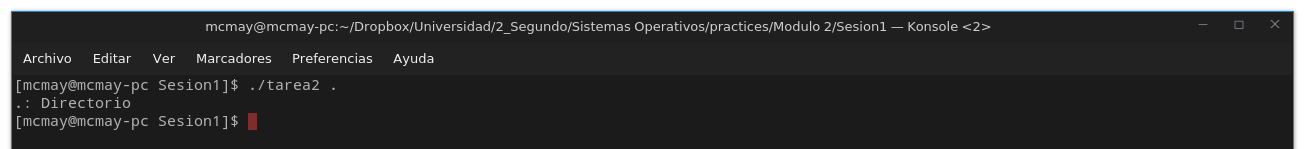
\includegraphics[width=1\linewidth]{image/ejer-03-A}
	\caption[Ejercicio 3.]{Resultado del ejecutable introduciendo el directorio origen}
	\label{fig:ejer-03-a}
\end{figure}

{\Large \textbf{Ejercicio 4.}} Define una macro en lenguaje C que tenga la misma funcionalidad que la macro
S\_ISREG(mode) usando para ello los flags definidos en <sys/stat.h> para el campo st\_mode de
la struct stat, y comprueba que funciona en un programa simple. Consulta en un libro de C o
en internet cómo se especifica una macro con argumento en C. \href{file: file/ejercicio_4.c}{\textcolor{Blue}{Descarga file}} \newline

El nuevo código que se pide, con las modificaciones realizadas: 

\lstset{language=, breaklines=true, basicstyle=\footnotesize}
\begin{lstlisting}[frame=single]
#include<unistd.h>  
#include<stdio.h>
#include<stdlib.h>
#include<sys/types.h>  
#include<sys/stat.h>
#include<stdio.h>
#include<errno.h>
#include<string.h>

//Parte A
#define S_ISREG2(mode) (((mode) & S_IFMT) == 0100000)

//Parte B
int main(int argc, char *argv[]) {
	int i;
	struct stat atributos;
	char tipoArchivo[30];
	
	if(argc<2) {
		printf("\nSintaxis de ejecucion: tarea2 [<nombre_archivo>]+\n\n");
		exit(EXIT_FAILURE);
	}
	
	for(i=1;i<argc;i++) {
		printf("%s: ", argv[i]);
		if(lstat(argv[i],&atributos) < 0) {
			printf("\nError al intentar acceder a los atributos de %s",argv[i]);
			perror("\nError en lstat");
		}
		else {
			if(S_ISREG2(atributos.st_mode)) strcpy(tipoArchivo,"Regular");
			else if(S_ISDIR2(atributos.st_mode)) strcpy(tipoArchivo,"Directorio");
			else if(S_ISCHR2(atributos.st_mode)) strcpy(tipoArchivo,"Especial de caracteres");
			else if(S_ISBLK2(atributos.st_mode)) strcpy(tipoArchivo,"Especial de bloques");
			else if(S_ISFIFO2(atributos.st_mode)) strcpy(tipoArchivo,"Tuberia con nombre (FIFO)");
			else if(S_ISLNK(atributos.st_mode)) strcpy(tipoArchivo,"Enlace relativo (soft)");
			else if(S_ISSOCK(atributos.st_mode)) strcpy(tipoArchivo,"Socket");
			else strcpy(tipoArchivo,"Tipo de archivo desconocido");
			printf("%s\n",tipoArchivo);
		}
	}
	
	return EXIT_SUCCESS;
}

\end{lstlisting}

Como se puede opserbar en el apartado A, se realiza la definición del nuevo S\_ISREG2. \newline

\begin{figure}[H]
	\centering
	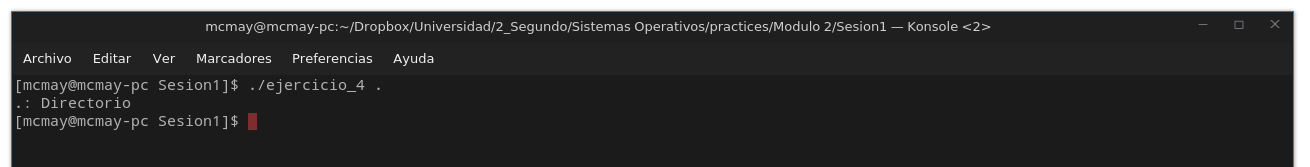
\includegraphics[width=1\linewidth]{image/ejer-04-A}
	\caption[Ejercicio 4.]{Resultado del ejecutable introduciendo el directorio origen}
	\label{fig:ejer-04-a}
\end{figure}

%----------------------------------------------------------------------------------------
%	Bibliografía
%----------------------------------------------------------------------------------------

%\footnote{Este es un ejemplo} comentario a pie de pagina

%palabra \cite{mrx05,prueba2}. realizacion de referencias

%\url dirección referenciar una url


%para que no falle la bibliografia hay que generar el fichero bibliografia.bib y tendran el siguiente formato dentro
	%@article{mrx05, 
	%auTHor = "Mr. X", 
	%Title = {Something Great}, 
	%publisher = "nob" # "ody", 
	%YEAR = 2005, 
	%} 


%------------------------------------------------
%\newpage
%\bibliography{bibliografia} %archivo citas.bib que contiene las entradas 
%\bibliographystyle{plain} % hay varias formas de citar

\end{document}
